\begin{frame}{Programación Eficiente}
    \begin{center}
        \fbox{\parbox[c]{.7\linewidth}{\emph{\textbf{Faster, better, cheaper,\\choose two of the above.}}\\.\hspace{2cm}Viejo proverbio de la ingeniería}}
    \end{center}

    \vspace{.5cm}Objetivo:
    \begin{itemize}
        \item identificar problemáticas que afectan la performance de un software
        \item adquirir técnicas y tácticas para optimización de código
        \item aprovechar la capacidad del hardware disponible
    \end{itemize}
\end{frame}

\begin{frame}{Programación Eficiente}
    Vamos a:
    \begin{itemize}
        \item Analizar código fuente
        \item Depurar código fuente
        \item Medir tiempos de ejecución
        \item Medir cobertura de código
        \item Estudiar interacción en
        \begin{itemize}
            \item Funciones
            \item Objetos
        \end{itemize}
    \end{itemize}
\end{frame}

\begin{frame}{Programación Eficiente}
    \begin{center}
        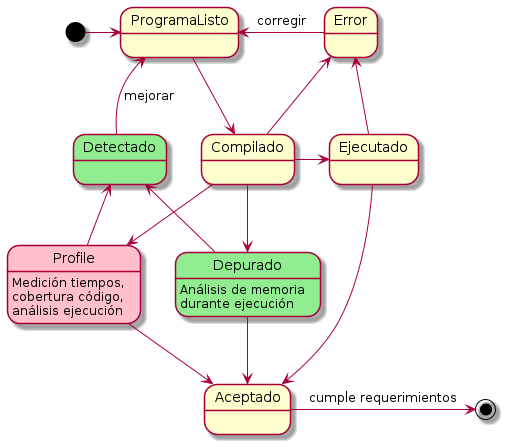
\includegraphics[scale=.5]{../imagenes/desarrolloSW.png}
    \end{center}
\end{frame}

\begin{frame}{Performance del Software}
    Al desarrollar software debemos:
    \begin{itemize}
        \item Aplicar buenas prácticas
        \item Evitar construcciones incorrectas
        \item Hacer un código claro
        \item Considerar el rol de compilador
        \item Hacer las pruebas necesarias
    \end{itemize}
\end{frame}

